%elatex
\documentclass[12pt]{extreport}
\usepackage[utf8]{inputenc}
\usepackage[T2A]{fontenc}
\usepackage[english,ukrainian]{babel}
%\usepackage{fontspec}
%\setmainfont{Nimbus Roman}
\usepackage{amsmath}
%\usepackage{mathspec}
%\usepackage{newtxmath}
%\setallmainfonts{Nimbus Roman}
\usepackage{graphicx}
\usepackage[a4paper,margin=0.5in]{geometry}
\pagestyle{empty}

\usepackage{pgfplots}
\pgfplotsset{compat=1.18}
\usetikzlibrary{intersections}
\usepackage{wrapfig}
\usepackage{indentfirst}
\usepackage{pdfpages}
\usepackage{caption}
\usepackage{subfiles}

\begin{document}
\includepdf[pages=-]{13tit.pdf}

\subsection*{Мета роботи}

Вивчити явище інтерференції і дифракції лазерного випромінювання, визначити:
а) довжину хвилі лазерного випромінювання; б) сталу дифракційної гратки

\subsection*{Прилади та обладнання}
Лазер неперервної дії (He-Ne лазер типу ЛГ-56),
мікрооб’єктив з екраном, плоскопаралельна
скляна пластинка, дифракційна гратка, циркуль

\subsection*{Теоретичні відомості та опис установки}
Схематично лабораторна установка для спостереження смуг
однакового нахилу і визначення довжини хвилі лазерного
випромінювання наведена на рис. 1.
Якщо на плоскопаралельну пластинку П спрямувати розбіжний
пучок світла, який формується мікрооб’єктивом О, то промені,
відбиті від передньої і задньої граней плоскопаралельної
пластинки є когерентними та інтерферують. Інтерференційна
картина у вигляді концентричних кілець – смуг однакового
нахилу спостерігається на екрані Е.

\begin{figure}[h]
	\centering
	
\includegraphics[width=.5\textwidth]{1.png}
	\caption{}
\end{figure}

Також, установивши дифракційну ґратку на місці мікрооб'єктива
та інший екран на місці плоскопаралельної пластинки, можна
спостерігати явище дифракції (рис. 2):

\begin{figure}[h]
	\centering
	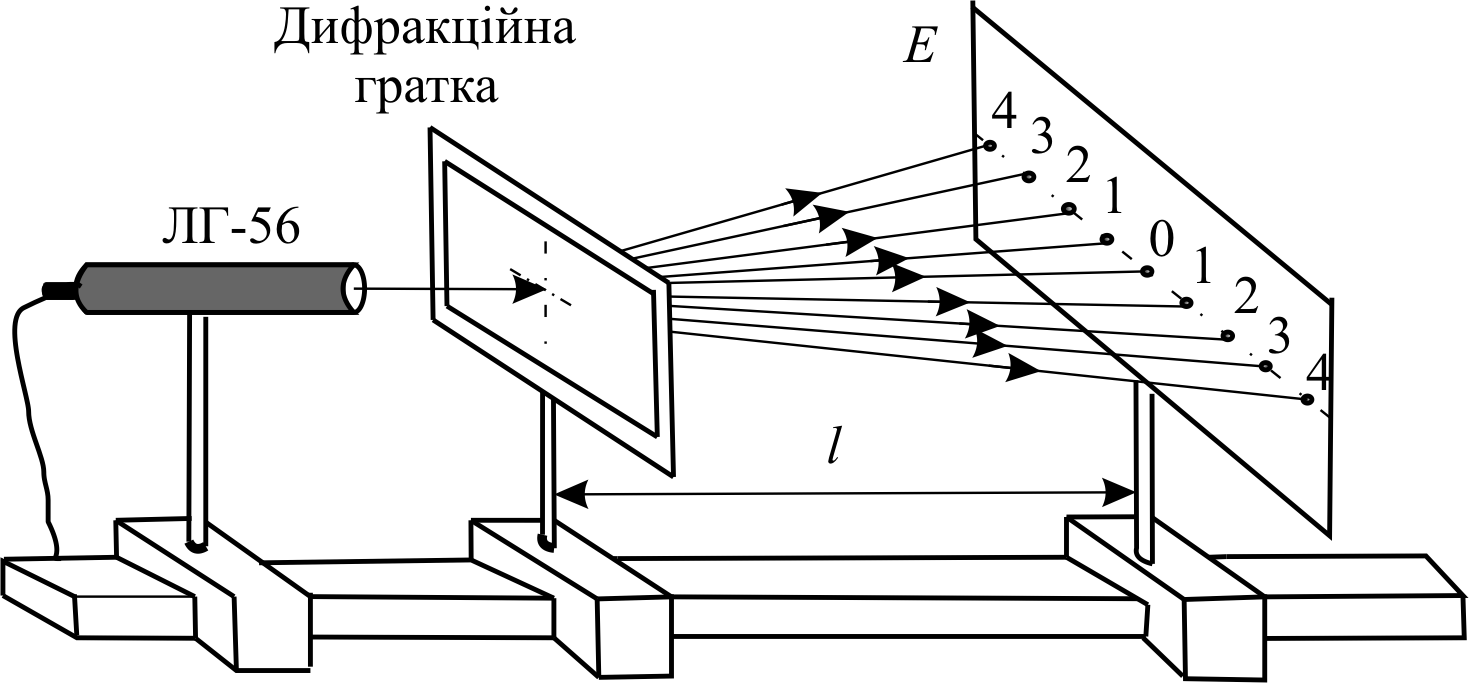
\includegraphics[width=.5\textwidth]{2.png}
	\caption{}
\end{figure}

\subsection*{Задані величини}
Товщина плоскопаралельної пластинки $d=0.0215$ \textit{м,}
показник заломлення скла $n=1.5$.

\subsection*{Фізичні величини, які вимірюються прямим способом}

$l, r_m, R$

\section*{Завдання 1}
\subsection*{{Таблиці результатів вимірювань}}

\renewcommand{\arraystretch}{1.3}
\begin{table}[h]
\caption{}
\centering
\begin{tabular}{|c| c| c| c| c| c| c|}
	\hline
	№ кільця, $m$ & 1 & 2 & 3 & 4 & 5\\
	\hline
	$r_m$, \textit{мм} & 3 & 4.4 & 5.1 & 7 & 8 \\
	\hline
	$r_m^2$, \textit{мм}$^2$ & 9 & 19.36 & 26.01 & 49 & 64 \\
	\hline
\end{tabular}
\end{table}
%======================================================================|
\begin{table}[h]
\caption{}
\centering
%\renewcommand{\arraystretch}{2.7}
\begin{tabular}{|c| c| c| c| c| c| c|}
	\hline
	№ з/п & $\left|\frac{\Delta r_{\Delta m}^2}{\Delta m}\right|,$
	\textit{мм}$^2$ & $R$, \textit{м} & $d,$ \textit{мм} &
	$\lambda_0,$ \textit{нм} & $\Delta\lambda_0,$ \textit{нм} &
	$\delta\lambda_0,$ \% \\
	\hline
	1 & 13.75 & 0.264 & & 682.55 & 38.3882 & \\
	\cline{1-3} \cline{5-6}
	2 & 14.82 & 0.269 & 21.5 & 735.6648 & 91.5030 & 13.4429\\
	\cline{1-3} \cline{5-6}
	3 & 18.995 & 0.273 & & 514.2704 & 129.8913 & \\
	\cline{1-3} \cline{5-6}
	\textit{сер.} & 15.855 & 0.26866 & & 644.1617(3) & 86.5941(6) & \\
	\hline
\end{tabular}
\end{table}
\subsection*{Графік залежності $r^2_m$ від \textit{m}, обчислення значення кутового коефіцієнта}

\begin{figure}[h]
	\centering
	\subfile{plot.tex}
	\caption{}
\end{figure}

\begin{equation}
	\begin{aligned}
		\Delta m_{1,5} = 4,~
		\Delta r_{\Delta m_{1,5}}^2=64-9=55,\\
		\left|\frac{\Delta r_{\Delta m_{1, 5}}^2}{\Delta m_{1, 5}}\right|
		=\frac{55}{4}=13.75;\\
		\Delta m_{2,4} = 2,~
		\Delta r_{\Delta m_{1,5}}^2=49-19.36 = 29.64,\\
		\left|\frac{\Delta r_{\Delta m_{2, 4}}^2}{\Delta m_{2, 4}}\right|
		=\frac{29.64}{2}=14.82;\\
		\Delta m_{3,5} = 2,~
		\Delta r_{\Delta m_{3,5}}^2=64-26.01 = 37.99,\\
		\left|\frac{\Delta r_{\Delta m_{1, 2}}^2}{\Delta m_{1, 2}}\right|
		=10.36;\\
	\end{aligned}
\end{equation}
%		1,9
%		2,19.36
%		3,26.01
%		4,49
%		5,64
\newpage
\subsection*{Обчислення шуканої величини за робочою формулою}
\begin{equation}
	\frac{d}{4nR^2}=21.5/(4\cdot1.5\cdot268.66^2)=0.00004964~[1/\text{мм}]\\
\end{equation}
	\begin{align}
		%\lambda_0 = \frac{d}{4nR^2}\cdot
		%\left|\frac{\Delta r_{\Delta m}^2}{\Delta m}\right|\\
		\lambda_{0_1} = \frac{d}{4nR^2}\cdot
		\left|\frac{\Delta r_{\Delta m_{1, 5}}^2}{\Delta m_{1, 5}}\right|=
		0.00004964\cdot13.75=0.00068255~[\text{мм}]=682.55~[\text{нм}]\\
		\lambda_{0_2} = \frac{d}{4nR^2}\cdot
		\left|\frac{\Delta r_{\Delta m_{2, 4}}^2}{\Delta m_{2, 4}}\right|=
		0.00004964\cdot14.82\cdot10^6=735.6648~[\text{нм}]\\
		\lambda_{0_3} = \frac{d}{4nR^2}\cdot
		\left|\frac{\Delta r_{\Delta m_{1, 2}}^2}{\Delta m_{1, 2}}\right|=
		0.00004964\cdot10.36\cdot10^6=514.2704~[\text{нм}]
	\end{align}
\subsection*{Обчислення похибок}
	\begin{equation}
		\Delta\lambda_{0_{cep}} =
		\frac{|644.16173-682.55|+|644.1...3-735.6648|+|644.1...3-514.2704|}{3} = 86.59416~[\text{нм}] \\
	\end{equation}
	\begin{equation}
		\delta\lambda_0 = 100\cdot86.59416/644.16173 = 13.4429~[\%].
	\end{equation}
%2222222222222222222222222222222222222222222222222222222222222222222222222222222222
%=================================================================================
%2222222222222222222222222222222222222222222222222222222222222222222222222222222222
\section*{Завдання 2}

\subsection*{{Таблиця результатів вимірювань}}
\begin{table}[h]
\caption{}
\centering
%\renewcommand{\arraystretch}{2.7}
\begin{tabular}{|c| c| c| c| c| c| c|c|}
	\hline
	№ з/п & $l,$ \textit{мм} & $\Delta l,$ \textit{мм} &
	$m$, & $r_m,$ \textit{мм}
	& $d,$ \textit{нм} & $\Delta d,$ \textit{нм} &
	$\delta d,$ \% \\
	\hline
	1 & 200 & 2.5 & 1 & 12 & 10809.8864 & 522.1469 & \\
	\cline{1-7}
	2 & 200 & 2.5 & 2 & 22 & 11792.6033 & 460.5699 & \\
	\cline{1-7}
	3 & 200 & 2.5 & 3 & 34 & 11445.762 & 113.7286 & 2.5339 \\
	\cline{1-7}
	4 & 200 & 2.5 & 4 & 46 & 11279.8814 & 52.1519 & \\
	\cline{1-7}
	\textit{сер.} & 200 & 2.5 & $xxxx$ & 23,5 & 11332.03334 & 287.1493 & \\
	\hline
\end{tabular}
\end{table}
\subsection*{Обчислення шуканої величини за робочою формулою}
%======================================================================|
	Стала дифракційної ґратки була обчислена за формулою (\ref{dst}):
	\begin{equation}
		d=\frac{m\lambda\sqrt{l^2+r_m^2}}{r_m}\\
		\label{dst}
	\end{equation}
	\begin{equation}
		\begin{aligned}
			d_1=\frac{1\cdot644.16173\sqrt{200^2+23.5^2}}
			{12} = 10809.8864~[\text{нм}]
			 \\
			d_2=\frac{2\cdot644.16173\sqrt{200^2+23.5^2}}
			{22} = 11792.6033~[\text{нм}]
			 \\
			d_3=\frac{3\cdot644.16173\sqrt{200^2+23.5^2}}
			{34} = 11445.7620~[\text{нм}]
			 \\
			d_4=\frac{4\cdot644.16173\sqrt{200^2+23.5^2}}
			{46} = 11279.8814~[\text{нм}]
			 \\
		\end{aligned}
	\end{equation}

	\begin{equation}
		d=11332.03334~\text{нм}.
	\end{equation}

\subsection*{Запис кінцевого результату}
$\lambda = (644.1617(3) \pm 86.5941(6))$ нм,
$d = (0.01133 \pm 0.0002871 $ мм.

%\end{center}
\subsection*{Аналіз кінцевих результатів та висновки}

Провівши цю лабораторну роботу, я визначив довжину хвилі випромінювання лазера,
застосувавши явище інтерференції, та, отримавши її, обчислив період дифракційної ґратки.

%{\fontsize{14}{16.2}\selectfont
\vspace{350pt}
{\fontsize{14}{16.2}\selectfont
Оцінка за виконання роботи:
\smallskip

\renewcommand{\arraystretch}{4}
\begin{tabular}{|c|c|c|}
	\hline
	\hspace{15pt} Допуск \hspace{15pt} & \hspace{15pt} Захист \hspace{15pt}
	& \hspace{15pt} Дата виконання \hspace{15pt}\\
	\hline
	 &  & \\
	\hline

\end{tabular}

\bigskip

	\begin{flushright}
		Підпис викладача:\line(1,0){70}\hspace{100pt}\hphantom{1pt}
	\end{flushright}
	}

\end{document}
